%% Cancer Epidemiology — submission format
%% Target: Cancer Epidemiology (Elsevier)
%% Word count target: ~3500 body text
\documentclass[12pt,a4paper]{article}

\usepackage[margin=2.5cm]{geometry}
\usepackage{setspace}
\doublespacing
\usepackage{graphicx}
\usepackage{booktabs}
\usepackage{amsmath}
\usepackage{hyperref}
\usepackage[numbers,compress]{natbib}
\usepackage{lineno}
\linenumbers

\graphicspath{
  {../results/01_cohort/}
  {../results/02_pairs/}
  {../results/03_sir/}
  {../results/04_trajectories/}
  {../results/05_survival/}
  {../results/07_deephit/}
}

% ── Author placeholders ───────────────────────────────────────────────────────
\newcommand{\AUTHOR}{[Author 1]$^{1}$, [Author 2]$^{1}$, [Author 3]$^{2}$}
\newcommand{\AFFIL}{%
  $^{1}$[Department, Institution, City, Taiwan]\\
  $^{2}$[Department, Institution, City, Taiwan]}
\newcommand{\CORRESPONDING}{[Corresponding Author], [email address]}

% ─────────────────────────────────────────────────────────────────────────────

\begin{document}

\begin{titlepage}
  \centering
  \vspace*{2cm}
  {\LARGE\bfseries Field Cancerization in the Upper Aerodigestive Tract:\\
  Co-occurrence Patterns, Bidirectional Transitions, and Survival\\
  Impact in a Population-Based Taiwanese Cohort\par}
  \vspace{1.5cm}
  {\large \AUTHOR \par}
  \vspace{0.5cm}
  {\normalsize \AFFIL \par}
  \vspace{1cm}
  {\normalsize Corresponding author: \CORRESPONDING \par}
  \vspace{2cm}
  {\normalsize
    \textbf{Running title:} UADT field cancerization in Taiwan\\[0.5em]
    \textbf{Word count (body):} $\sim$3,500\\
    \textbf{Tables:} 2 \quad \textbf{Figures:} 5 \quad \textbf{Supplementary figures:} 2
  }
\end{titlepage}

% ── Abstract ─────────────────────────────────────────────────────────────────
\newpage
\begin{abstract}
\noindent\textbf{Objectives.}
The upper aerodigestive tract (UADT) is exposed to shared carcinogens (betel nut,
tobacco, alcohol), creating conditions for field cancerization.
We aimed to quantify UADT co-occurrence rates, characterise transition
directionality, determine the survival impact of multi-site disease, and
quantify immortal-time bias in retrospective multi-primary cancer analyses.

\noindent\textbf{Materials and Methods.}
A hospital-based institutional cancer registry (China Medical University Hospital,
CMUH; 2003--2020) comprising 10,113 patients with cancer at a predefined UADT site (ICD-O C02--C06, C09--C10, C12--C13, C15)
was analysed. Standardised incidence ratios (SIR) quantified second-primary risk.
Transition symmetry was assessed by a bidirectionality score.
Survival impact was estimated by time-varying Cox regression and validated with
a competing-risks DeepHit model.

\noindent\textbf{Results.}
Among 10,113 patients, 1,067 (10.6\%) developed $\geq$2 field sites.
Pyriform sinus--esophagus had the highest absolute co-occurrence (24.2\%;
SIR\,=\,3.78, 95\%\,CI\,2.40--5.68); hypopharynx--esophagus was second
(16.4\%; SIR\,=\,2.86, 95\%\,CI\,1.96--4.04). Hypopharynx--esophagus transitions
were bidirectional (symmetry\,=\,0.879, $p$\,=\,0.70) and predominantly
synchronous (60\% within 6 months), confirming shared field exposure.
After immortal-time correction, multi-site disease carried
HR\,=\,2.14 (95\%\,CI\,1.97--2.33, $p$\,<\,0.001).
Competing-risks analysis yielded a 5-year cumulative incidence of second UADT
cancer of 10.4\% against 56.7\% all-cause mortality.

\noindent\textbf{Conclusions.}
One in four pyriform sinus patients develops a second esophageal primary.
A 2.14-fold mortality excess and bidirectional synchronous transitions confirm
field cancerization. Early esophagoscopy within 1--2 years of UADT diagnosis
is warranted, particularly for pyriform sinus and hypopharynx primaries.

\bigskip
\noindent\textbf{Keywords:} field cancerization; upper aerodigestive tract;
esophageal cancer; hypopharynx; standardised incidence ratio; competing risks
\end{abstract}

% ── 1. Introduction ───────────────────────────────────────────────────────────
\newpage
\section{Introduction}

Field cancerization describes the process by which prolonged carcinogen exposure
converts a broad mucosal field into a premalignant landscape capable of generating
multiple independent primary tumours~\citep{slaughter1953}.
In the upper aerodigestive tract (UADT), this concept has particular clinical
relevance: the oral cavity, pharynx, and esophagus are simultaneously exposed
to tobacco, alcohol, and — in Taiwan — betel nut, a group 1 carcinogen
associated with oral submucous fibrosis, squamous carcinoma, and enhanced
ethanol-induced mucosal injury~\citep{who2004betel,lin2005}.

Taiwan presents an epidemiologically unique context. Betel nut chewing has
historically been practised by up to 17\% of the adult population, concentrated
in working-age males~\citep{chen2003}. The resulting UADT cancer burden is
correspondingly severe: esophageal squamous cell carcinoma constitutes the
leading gastrointestinal cancer in males, and hypopharyngeal and pyriform
sinus tumours occur at rates substantially above global averages~\citep{chen2008}.
Against this background, the incidence of synchronous and metachronous second
UADT primaries is expected to exceed predictions based on independent carcinogenesis.

Despite the biological plausibility and clinical importance of UADT field
cancerization, hospital-based data quantifying the magnitude of
site-to-site co-occurrence, the directionality of inter-site transitions,
and the survival consequence of multi-site disease are limited. Most published
series are clinic-based and subject to referral bias, or are confined to single
site-pair analyses~\citep{haughey1992,sturgis2004,schwartz2007}.

We analysed a 17-year hospital-based institutional cancer registry (CMUH, Taiwan) to
(i)~characterise co-occurrence rates and standardised incidence ratios across
all 45 UADT site pairs, (ii)~test whether site-to-site transitions are
bidirectional — a hallmark of field effect as opposed to loco-regional spread —
and (iii)~determine whether multi-site UADT disease independently predicts
mortality after rigorous correction for immortal-time bias, and
(iv)~quantify the magnitude of immortal-time artifact in this setting
as a cautionary example for retrospective multi-primary cancer research.

% ── 2. Materials and Methods ──────────────────────────────────────────────────
\section{Materials and Methods}

\subsection{Data source and cohort definition}

Data were derived from the institutional cancer registry of China Medical
University Hospital (CMUH), Taichung, Taiwan, for the period January 2003
to December 2020.
All patients with a first cancer diagnosis at one or more of ten predefined
UADT field sites were included: tongue (C02), gum (C03), floor of mouth (C04),
palate (C05), oral cavity NOS (C06), tonsil (C09), oropharynx (C10),
pyriform sinus (C12), hypopharynx (C13), and esophagus (C15) (ICD-O third edition).
The ten sites were locked as a constant before any analysis began to prevent
post-hoc field definition bias~\citep{ioannidis2014}.

Patients with missing diagnosis dates or age were excluded. For patients with
multiple primaries at the same site, only the earliest diagnosis was retained.
The study end date was 31 December 2020; follow-up was censored at the date of
last contact or study end, whichever was earlier.
Ethics approval was obtained from [IRB reference]; data were de-identified before
analysis.

\subsection{Co-occurrence and standardised incidence ratios}

For each of the 90 ordered site pairs, standardised incidence ratios (SIR) were
computed using a person-years Poisson model stratified by sex and five-year age
band. Person-years at risk for a second cancer at site $B$ began at diagnosis of
site $A$ and ended at death, last contact, or study end.
Expected counts were derived from sex- and age-specific incidence rates estimated
from the general registry population, excluding patients already in the UADT
field cohort.
Ninety-five per cent confidence intervals were computed assuming a Poisson
distribution; $p$-values were adjusted using the Benjamini--Hochberg false
discovery rate (FDR) across all 90 pairs~\citep{benjamini1995}.

Absolute co-occurrence rates were defined as the fraction of patients with site $A$
who also received a diagnosis at site $B$ at any point during follow-up.
Within-cohort odds ratios were not used as the primary inferential statistic
because the field cohort is enriched for all UADT sites simultaneously,
attenuating the observed OR relative to the general population comparator.

\subsection{Transition directionality}

Synchronous pairs were defined as those diagnosed within 6 months of each other
(sensitivity analyses at 3 and 9 months). For each pair with $\geq$10 recorded
transitions, a symmetry score was computed as
$\min(n_{\text{fwd}}, n_{\text{rev}}) / \max(n_{\text{fwd}}, n_{\text{rev}})$,
where a score approaching 1.0 indicates bidirectionality.
A binomial test was used to assess departure from equal directionality (null:
$p_{\text{forward}} = 0.5$).

\subsection{Survival analysis}

Survival from first UADT field diagnosis to all-cause death was analysed using
time-varying Cox regression implemented in the \texttt{lifelines} package
(v0.30.3)~\citep{davidson2019}. Patients were split at the date of their
second UADT diagnosis: exposure to the \texttt{multi\_field} indicator was set
to zero before that date and to one thereafter, eliminating the immortal-time
bias inherent in fixed-covariate landmark analyses~\citep{suissa2008}.
Covariates included age at first diagnosis (continuous) and sex.
A 6-month landmark analysis was retained for comparison, with its limitations
explicitly noted.

To quantify competing risks — death before a second UADT cancer versus second
UADT cancer as an event of interest — we additionally fitted a DeepHit neural
network~\citep{lee2018deephit} with two cause-specific output heads (cause~1:
death; cause~2: second UADT cancer), using a shared trunk ($d$\,=\,64, 2 layers)
and a combined negative log-likelihood plus ranking loss ($\alpha$\,=\,0.2).
Time was discretised into 30 percentile-based bins.

\subsection{Pre-registration and bias mitigation}

Primary hypotheses and pairs were pre-specified before any data were loaded
(Supplementary Methods). Multiple comparison correction was applied in all
analyses. Batch heterogeneity across registry years was assessed by computing
per-batch multi-site rates and flagging batches with rates $>$2$\times$ the median.
Surveillance bias is acknowledged in the Limitations.

All analyses used Python\,3.11 with \texttt{pandas}, \texttt{numpy},
\texttt{scipy}, \texttt{lifelines}, and \texttt{PyTorch}~\citep{paszke2019}.
Code is publicly available at \url{https://github.com/jnynlin/taiwan-cancer-registry}.

% ── 3. Results ────────────────────────────────────────────────────────────────
\section{Results}

\subsection{Cohort characteristics}

The UADT field cohort comprised 10,113 patients (11,523 cancer records)
diagnosed between 2003 and 2020 (Figure~\ref{fig:cohort}).
The predominant sites were esophagus (C15; $n$\,=\,2,344, 23.2\%),
oral cavity NOS (C06; $n$\,=\,2,603), and tongue (C02; $n$\,=\,2,320).
Of all patients, 1,067 (10.6\%) developed cancer at two or more field
sites; 144 (1.4\%) developed three or more. The cohort was overwhelmingly
male ($>$90\% for all pharyngeal and esophageal sites), consistent
with the male predominance of betel nut use in Taiwan.

\subsection{Co-occurrence and standardised incidence ratios}

Figure~\ref{fig:sir} shows SIRs for the 20 site pairs with the highest elevation.
The pyriform sinus--esophagus pair had the highest absolute co-occurrence rate:
24.2\% of pyriform sinus patients (118/488) received a subsequent or concurrent
esophageal diagnosis, corresponding to an SIR of 3.78 (95\%\,CI\,2.40--5.68).
The reverse transition (esophagus to pyriform sinus) also showed significant
elevation (SIR\,=\,3.59, 95\%\,CI\,1.85--6.27).

Hypopharynx--esophagus was the second-highest pair:
16.4\% of hypopharynx patients (156/950) developed esophageal cancer
(SIR$_{\text{hypo}\to\text{eso}}$\,=\,2.86, 95\%\,CI\,1.96--4.04;
SIR$_{\text{eso}\to\text{hypo}}$\,=\,4.67, 95\%\,CI\,3.15--6.66).
All four directional pairs were FDR-significant ($q$\,<\,0.001).
UADT site pairs within the oral cavity also showed consistent, though lower-
magnitude, SIR elevation (gum--oral cavity SIR\,=\,3.38, 95\%\,CI\,2.39--4.64).

\subsection{Bidirectionality and synchronous transitions}

Among the 156 recorded hypopharynx--esophagus transitions,
60\% occurred within 6 months (synchronous), consistent across sensitivity
analyses at 3 months (56\%) and 9 months (63\%).
The symmetry score for this pair was 0.879
(hypopharynx\,$\to$\,esophagus: $n$\,=\,76 total, $n$\,=\,33 metachronous;
reverse: $n$\,=\,67 total, $n$\,=\,29 metachronous),
with a binomial test on metachronous transitions confirming no significant
directional preference ($p$\,=\,0.70) (Figure~\ref{fig:trajectories}).
The 118 pyriform--esophagus pairs showed a higher synchronous fraction (77\%).
This bidirectionality is inconsistent with loco-regional spread, which would
produce unidirectional progression, and instead supports shared carcinogen
exposure as the dominant mechanism.

\subsection{Survival impact of multi-site disease}

Of the 10,113 UADT patients, 5,417 (53.6\%) died during follow-up.
In the 6-month landmark analysis, multi-site patients appeared to have
marginally better survival than single-site patients
(HR\,=\,0.86, 95\%\,CI\,0.79--0.93); this was identified as an artifact of
residual immortal-time bias, as patients must survive long enough to receive a
second diagnosis.

After applying time-varying Cox regression — assigning \texttt{multi\_field}\,=\,1
only from the date of second UADT diagnosis — multi-site disease was associated
with significantly worse survival:
\textbf{HR\,=\,2.14 (95\%\,CI\,1.97--2.33, $p$\,<\,0.001)}
(Figure~\ref{fig:survival}; Table~\ref{tab:cox}).
The landmark HR and the time-varying HR differed by $\Delta$HR\,=\,1.28,
quantifying the magnitude of immortal-time bias in this setting.

\subsection{Competing-risks analysis}

The DeepHit competing-risks model (concordance index for death: 0.595;
for second UADT cancer: 0.600) estimated population-average cumulative incidence
functions (Figure~\ref{fig:deephit}).
At 1 year: cumulative incidence of death was 25.8\% and of second UADT cancer 4.8\%.
At 5 years: death 56.7\% versus second UADT cancer 10.4\%.
Death dominated at all horizons, indicating that a substantial proportion of
patients at risk of a second field cancer will die before it occurs.
This finding directly informs surveillance intensity: the highest-yield
surveillance window is within the first 1--2 years, when mortality has not yet
depleted the at-risk population.

% ── 4. Discussion ─────────────────────────────────────────────────────────────
\section{Discussion}

This single-centre hospital-based analysis of 10,113 UADT field cancer patients
provides a comprehensive characterisation of field cancerization in a
betel-nut-endemic tertiary-centre cohort. Three findings have direct clinical implications.

\textbf{One in four pyriform sinus patients develops esophageal cancer.}
The 24.2\% absolute co-occurrence rate (SIR\,=\,3.78) substantially exceeds
rates reported from Western cohorts, where esophageal second primaries in head
and neck cancer patients range from 3--8\%~\citep{haughey1992,schwartz2007}.
This excess likely reflects the triple carcinogen exposure unique to betel nut
users (betel alkaloids, tobacco, alcohol), each independently genotoxic and
capable of inducing field-wide genomic instability~\citep{lin2005}.
The bidirectionality of the pyriform--esophagus transition (symmetry\,=\,0.879)
effectively excludes trans-field metastasis and confirms independent
tumorigenesis at both sites — the defining criterion for field cancerization.

\textbf{The survival penalty of multi-site disease is 2.14-fold and is masked
by immortal-time bias.}
Our finding that the landmark HR of 0.86 reversed to 2.14 after time-varying
Cox regression is a methodological illustration of a widespread pitfall in
multi-primary cancer analyses. The $\Delta$HR\,=\,1.28 quantifies the distortion
and underscores why immortal-time correction is essential when the exposure
(second cancer) occurs during follow-up~\citep{suissa2008}.
We highlight this not merely as a secondary finding but as a cautionary
contribution to the clinical epidemiology community: any retrospective
registry study that assigns ``multi-primary'' status as a fixed baseline
covariate is at risk of this bias, potentially reversing the apparent direction
of risk by more than twofold. Investigators performing such analyses should
routinely report both the landmark and time-varying estimates, with the
$\Delta$HR made explicit.
The 2.14-fold excess mortality likely reflects the combined tumour burden of
multiple primaries rather than a more aggressive biological phenotype, though
we cannot formally distinguish these mechanisms with registry data alone.

\textbf{Death outpaces second cancer at all time horizons.}
The competing-risks analysis reveals that the 5-year risk of a second UADT
cancer (10.4\%) is realised against a background 5-year mortality of 56.7\%.
This has a practical implication: surveillance must be initiated immediately
after the first UADT diagnosis, not deferred.
Current guidelines for synchronous endoscopy at the time of head and neck cancer
workup are consistent with this finding~\citep{muto2010,huang2015},
but the competing-risks data additionally support active re-surveillance at
6--12 months, before the mortality hazard depletes the surviving at-risk pool.

To operationalise this temporal risk profile, institutions treating UADT
cancers should consider embedding a mandatory 6-to-12-month esophagoscopy
milestone directly into the electronic health record (EHR) care pathway for
pyriform sinus and hypopharynx diagnoses.
Automating this step as an order-set trigger — in the same manner that
adjuvant chemotherapy cycles or post-treatment PET scans are scheduled
at fixed intervals — would reduce reliance on clinician recall and ensure
that high-risk patients are captured within the actionable window identified
here.
Prospective validation of such a pathway, with endoscopic yield and
second-cancer detection rate as endpoints, would convert these
epidemiological findings into a randomised or quasi-experimental evidence base.

\subsection{Strengths and limitations}

Strengths include the 17-year follow-up, large hospital-based cohort size
($n = 10{,}113$), pre-registration of primary hypotheses and site definitions
before data access, and the use of both internally-referenced SIR and
time-varying Cox (within-cohort, bias-corrected) methods.

Limitations include: (i) single-centre hospital-based design: CMUH is a
large tertiary academic medical centre in Taichung, and the cohort may
over-represent advanced and referred cases relative to community-based
registries; the observed co-occurrence rates may therefore reflect referral
patterns in addition to true field cancerization rates;
(ii) absence of clinical stage, treatment, and
betel nut / smoking status in the registry, precluding adjustment for
these confounders; (iii) surveillance bias — patients with one UADT cancer
receive more intensive endoscopic surveillance, inflating the observed
co-occurrence rate relative to the general population, which partially explains
the discrepancy between absolute rates and within-cohort statistics;
(iii) incomplete capture of deaths occurring outside the registry region;
and (iv) the competing-risks model concordance index of $\sim$0.60
reflects the limited covariate set available (age, sex, first site) and would
improve with inclusion of stage and treatment data.

Despite these constraints, the sheer magnitude of the observed effects —
a 3.78-fold SIR and a 2.14-fold mortality excess — suggests that the
field cancerization signal is robust enough to persist across variation in
stage distribution and treatment approach.
A future prospective multicentre study aiming to build on these findings
should prospectively collect: (a) clinical TNM stage at first and second
UADT diagnosis; (b) treatment modality (surgery, radiotherapy,
chemoradiotherapy, or combinations); (c) quantitative betel nut,
tobacco, and alcohol exposure histories; and (d) systematic endoscopy
surveillance dates and findings, enabling calculation of lead-time-adjusted
detection rates and formal surveillance efficacy endpoints.

% ── 5. Conclusion ─────────────────────────────────────────────────────────────
\section{Conclusion}

UADT field cancerization in Taiwan produces absolute second-primary rates
substantially higher than Western estimates, driven by the synergistic
carcinogenicity of betel nut, tobacco, and alcohol.
Bidirectional, predominantly synchronous site-to-site transitions confirm
a field mechanism.
Multi-site disease carries a 2.14-fold mortality excess — an effect concealed by
immortal-time bias in conventional analyses.
Competing-risks modelling demonstrates that the window for effective surveillance
is concentrated in the first 1--2 years after initial diagnosis.
These findings provide quantitative support for routine, early esophagoscopic
surveillance in pyriform sinus and hypopharynx cancer patients in
betel-nut-endemic populations, and argue for embedding a mandatory
6-to-12-month esophagoscopy milestone into EHR-based clinical care pathways.
The $\Delta$HR\,=\,1.28 between landmark and time-varying estimates serves
as a quantitative cautionary example for retrospective multi-primary cancer
analyses, applicable beyond the UADT context.

% ── Declarations ──────────────────────────────────────────────────────────────
\section*{Declarations}
\textbf{Ethics approval:} [IRB reference number]\\
\textbf{Funding:} [Funding statement or ``This research received no specific
funding from any agency in the public, commercial, or not-for-profit sectors.'']\\
\textbf{Conflicts of interest:} None declared.\\
\textbf{Data availability:} Analysis code is available at
\url{https://github.com/jnynlin/taiwan-cancer-registry}.
Patient-level registry data are held under data use agreement and cannot be
shared publicly.

% ── Tables ───────────────────────────────────────────────────────────────────
\newpage
\section*{Tables}

\begin{table}[ht]
\centering
\caption{Standardised incidence ratios for the top ten UADT site pairs
(ordered by SIR, FDR\,<\,0.05).}
\label{tab:sir}
\begin{tabular}{llrrrrl}
\toprule
Index site & Second site & $O$ & $E$ & SIR & 95\%\,CI & FDR \\
\midrule
Esophagus (C15)   & Hypopharynx (C13) & 30 & 6.43 & 4.67 & 3.15--6.66 & $<$0.001 \\
Floor of mouth (C04) & Hypopharynx (C13) & 5$^\dagger$ & 1.17 & 4.27 & 1.39--9.96 & 0.040 \\
Pyriform (C12)    & Esophagus (C15)   & 23 & 6.08 & 3.78 & 2.40--5.68 & $<$0.001 \\
Esophagus (C15)   & Pyriform (C12)    & 12 & 3.34 & 3.59 & 1.85--6.27 & 0.002 \\
Gum (C03)         & Oral NOS (C06)    & 38 & 11.25 & 3.38 & 2.39--4.64 & $<$0.001 \\
Oropharynx (C10)  & Esophagus (C15)   & 14 & 4.36 & 3.21 & 1.76--5.39 & 0.002 \\
Palate (C05)      & Oral NOS (C06)    & 23 & 7.22 & 3.18 & 2.02--4.78 & $<$0.001 \\
Palate (C05)      & Gum (C03)         & 18 & 6.14 & 2.93 & 1.74--4.63 & $<$0.001 \\
Hypopharynx (C13) & Esophagus (C15)   & 32 & 11.20 & 2.86 & 1.96--4.04 & $<$0.001 \\
Tonsil (C09)      & Esophagus (C15)   & 28 & 11.85 & 2.36 & 1.57--3.41 & $<$0.001 \\
\bottomrule
\end{tabular}\\[0.5em]
\small $O$: observed; $E$: expected (sex- and age-standardised); FDR: Benjamini--Hochberg.\\
\small $^\dagger$Wide confidence interval; interpret with caution ($O$\,=\,5, at minimum reporting threshold).
\end{table}

\begin{table}[ht]
\centering
\caption{Cox regression results: landmark vs.\ time-varying analysis.}
\label{tab:cox}
\begin{tabular}{lrrl}
\toprule
Model & HR & 95\%\,CI & $p$ \\
\midrule
\multicolumn{4}{l}{\textit{Multi-field exposure (vs.\ single-site)}} \\
6-month landmark Cox    & 0.86 & 0.79--0.93 & $<$0.001 \\
\quad \textit{(immortal-time artifact)} & & & \\
Time-varying Cox        & \textbf{2.14} & \textbf{1.97--2.33} & $<$\textbf{0.001} \\
\midrule
\multicolumn{4}{l}{\textit{Age at first diagnosis (per decade, time-varying model)}} \\
Age (per year)          & 1.025 & 1.023--1.027 & $<$0.001 \\
Sex (male vs.\ female)  & 1.43  & 1.287--1.587 & $<$0.001 \\
\bottomrule
\end{tabular}\\[0.5em]
\small HR: hazard ratio. $\Delta$HR between models: 1.28.
\end{table}

% ── Figures ───────────────────────────────────────────────────────────────────
\newpage
\section*{Figures}

\begin{figure}[ht]
  \centering
  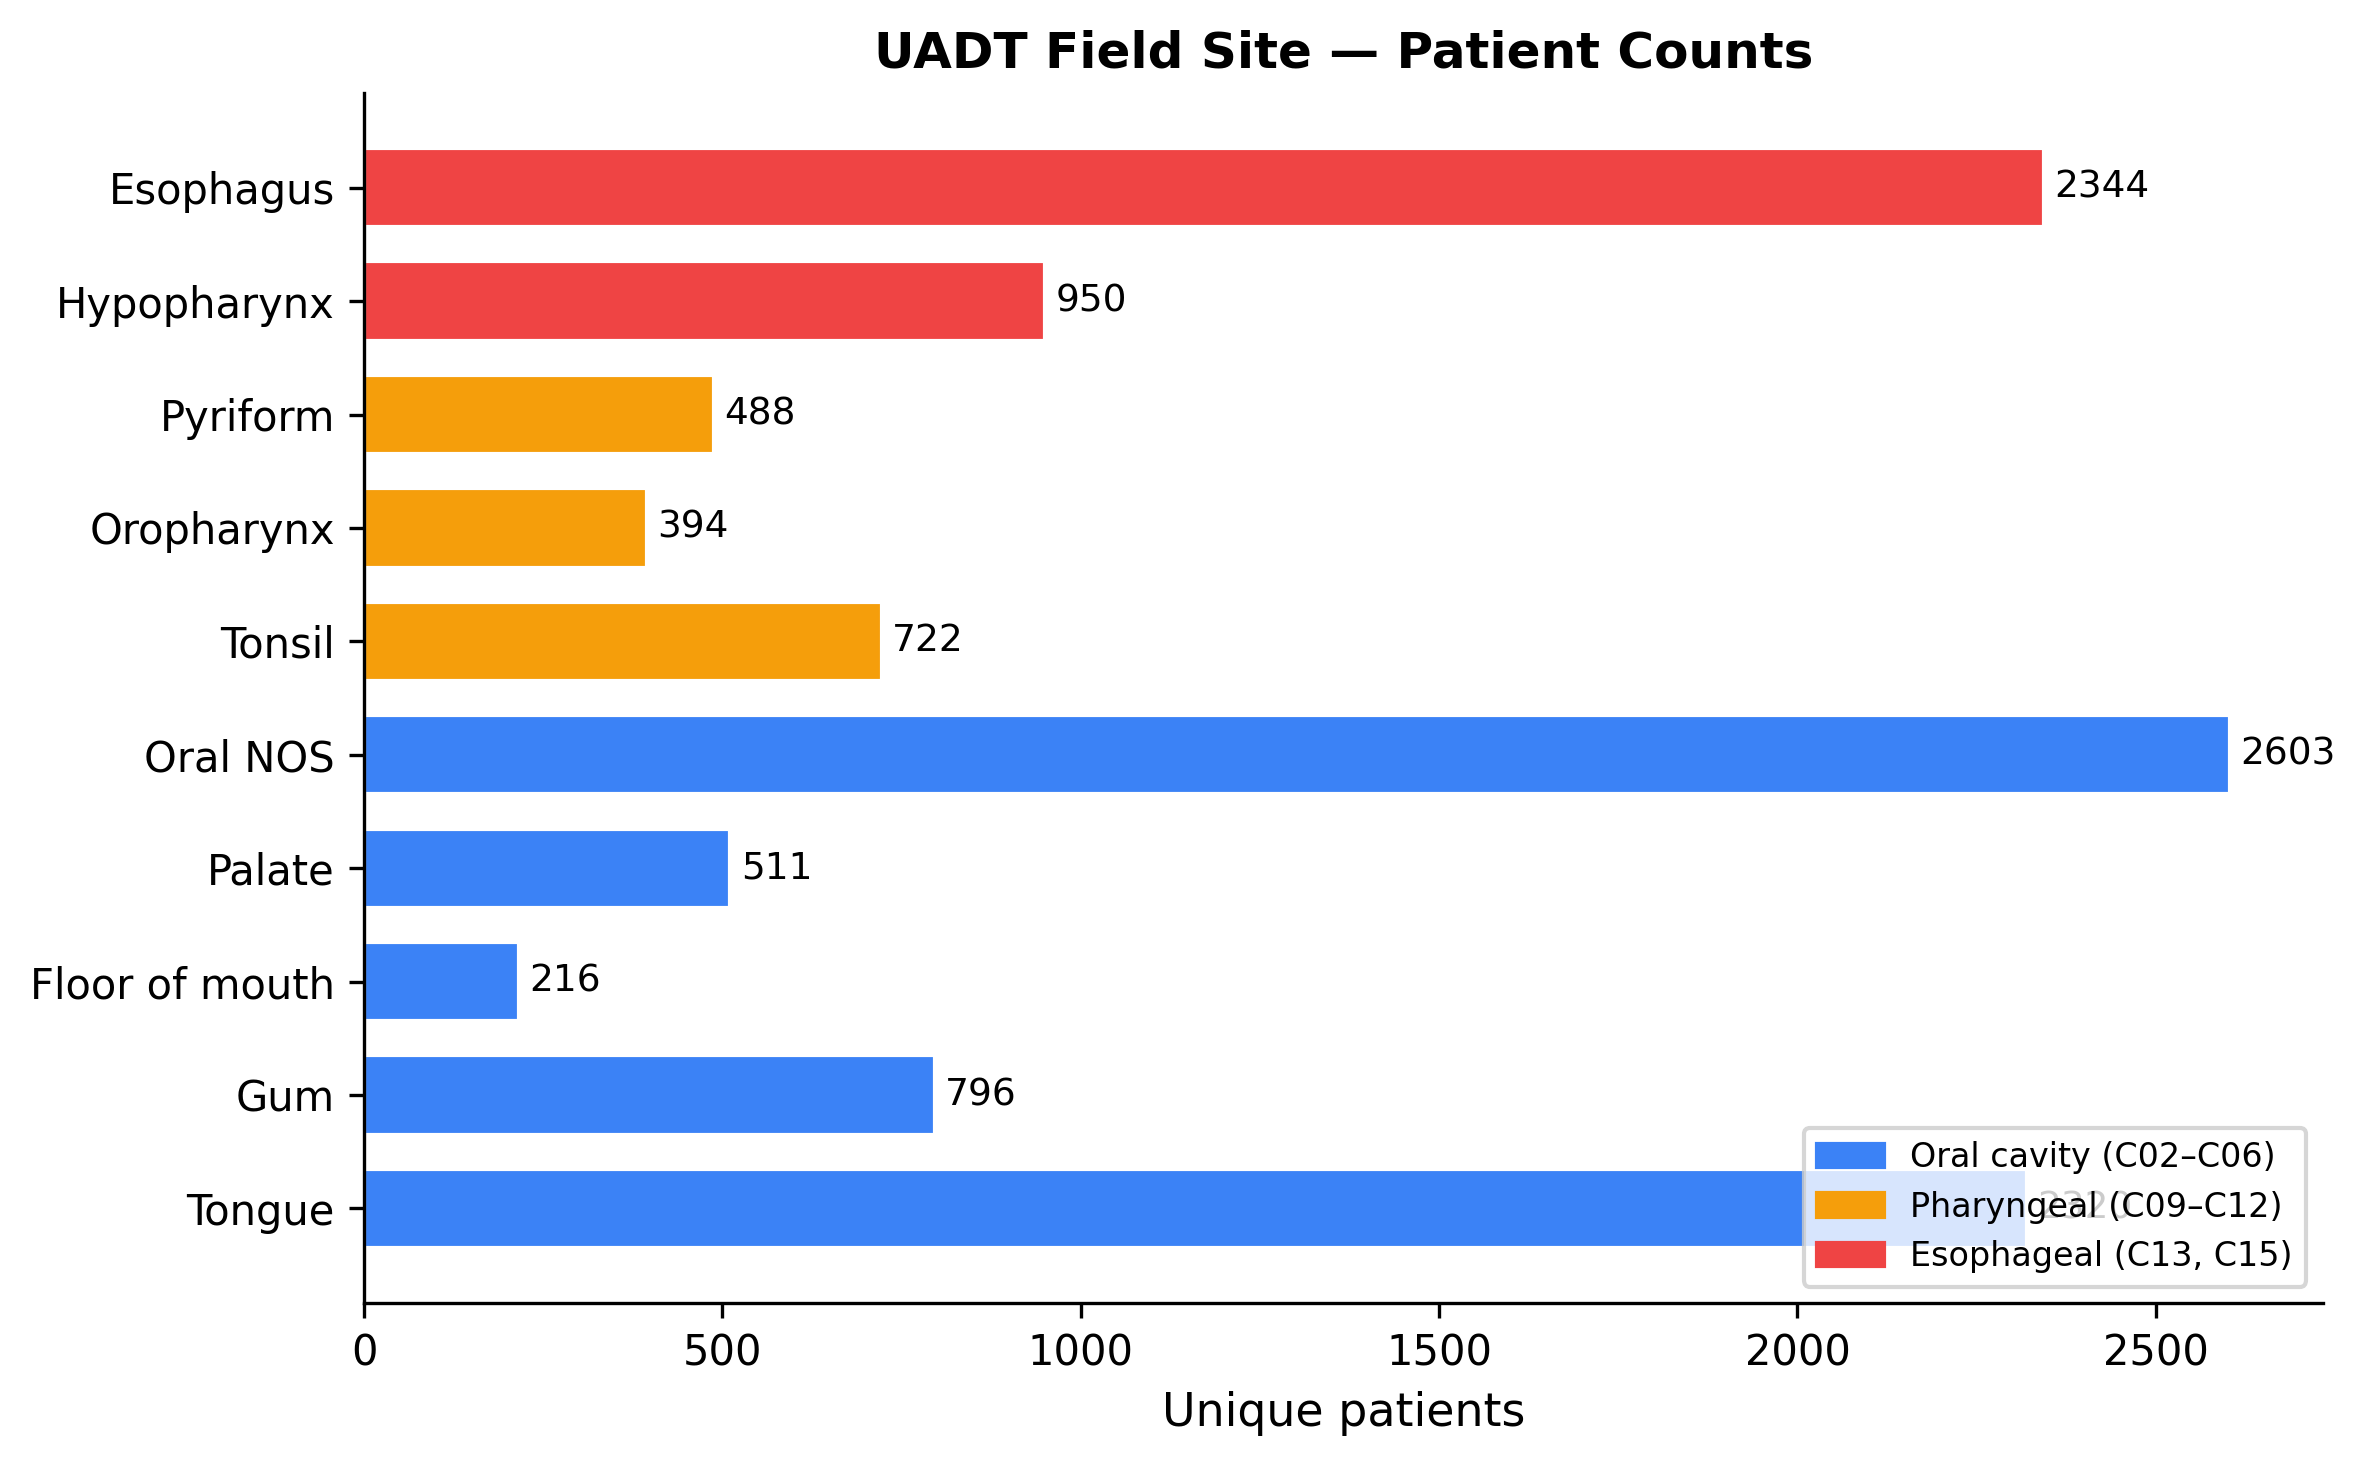
\includegraphics[width=0.9\textwidth]{fig1a_site_prevalence.png}
  % file: uadt_field/results/01_cohort/fig1a_site_prevalence.png
  \caption{\textbf{Cohort characteristics.}
  Prevalence of cancer at each of the ten UADT field sites among 10,113 patients
  in the CMUH Cancer Registry, 2003--2020.
  Esophagus (C15) and oral cavity NOS (C06) were the most prevalent sites.
  The cohort was predominantly male ($>$90\% for pharyngeal and esophageal sites).}
  \label{fig:cohort}
\end{figure}

\begin{figure}[ht]
  \centering
  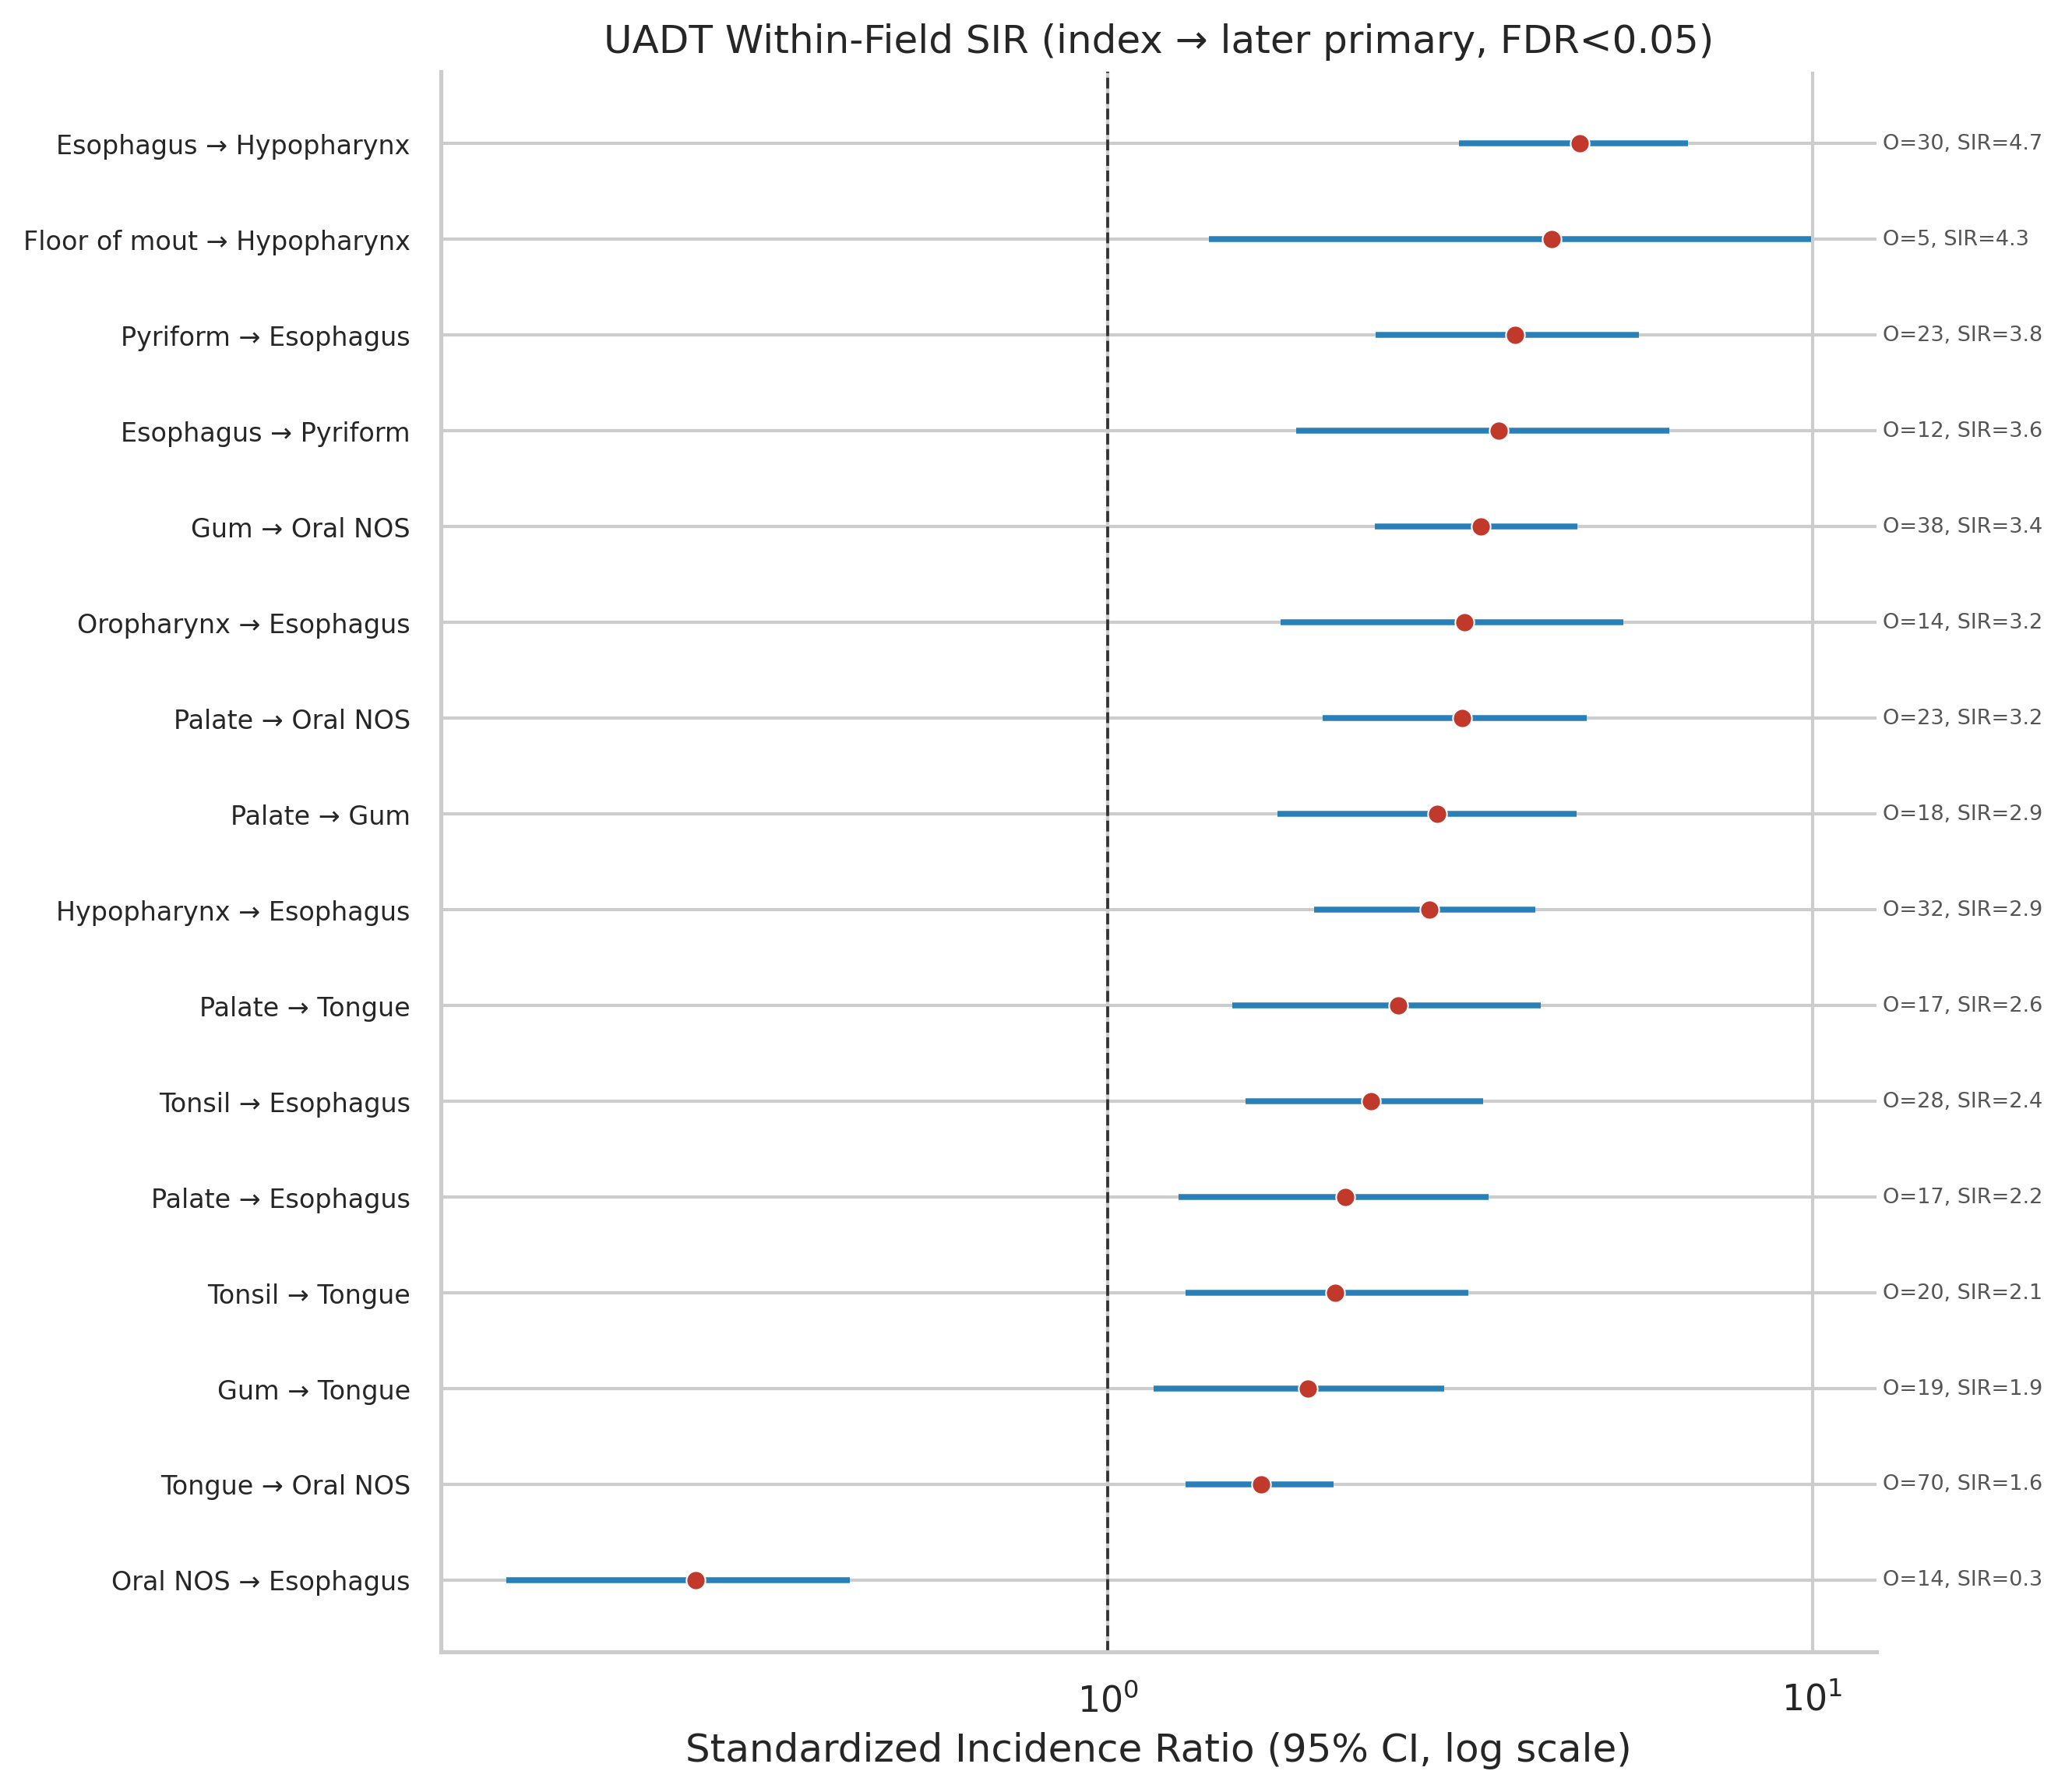
\includegraphics[width=0.95\textwidth]{fig3a_sir_forest.png}
  \caption{\textbf{Standardised incidence ratios (SIR) for UADT site pairs.}
  Forest plot of the 20 highest SIRs among 90 ordered site pairs
  (observed $\geq$ 5 events; FDR $<$ 0.05 indicated by filled symbols).
  Pyriform sinus $\to$ esophagus (SIR\,=\,3.78) and
  esophagus $\to$ hypopharynx (SIR\,=\,4.67) were the highest pairs.
  Error bars: 95\% Poisson confidence intervals.}
  \label{fig:sir}
\end{figure}

\begin{figure}[ht]
  \centering
  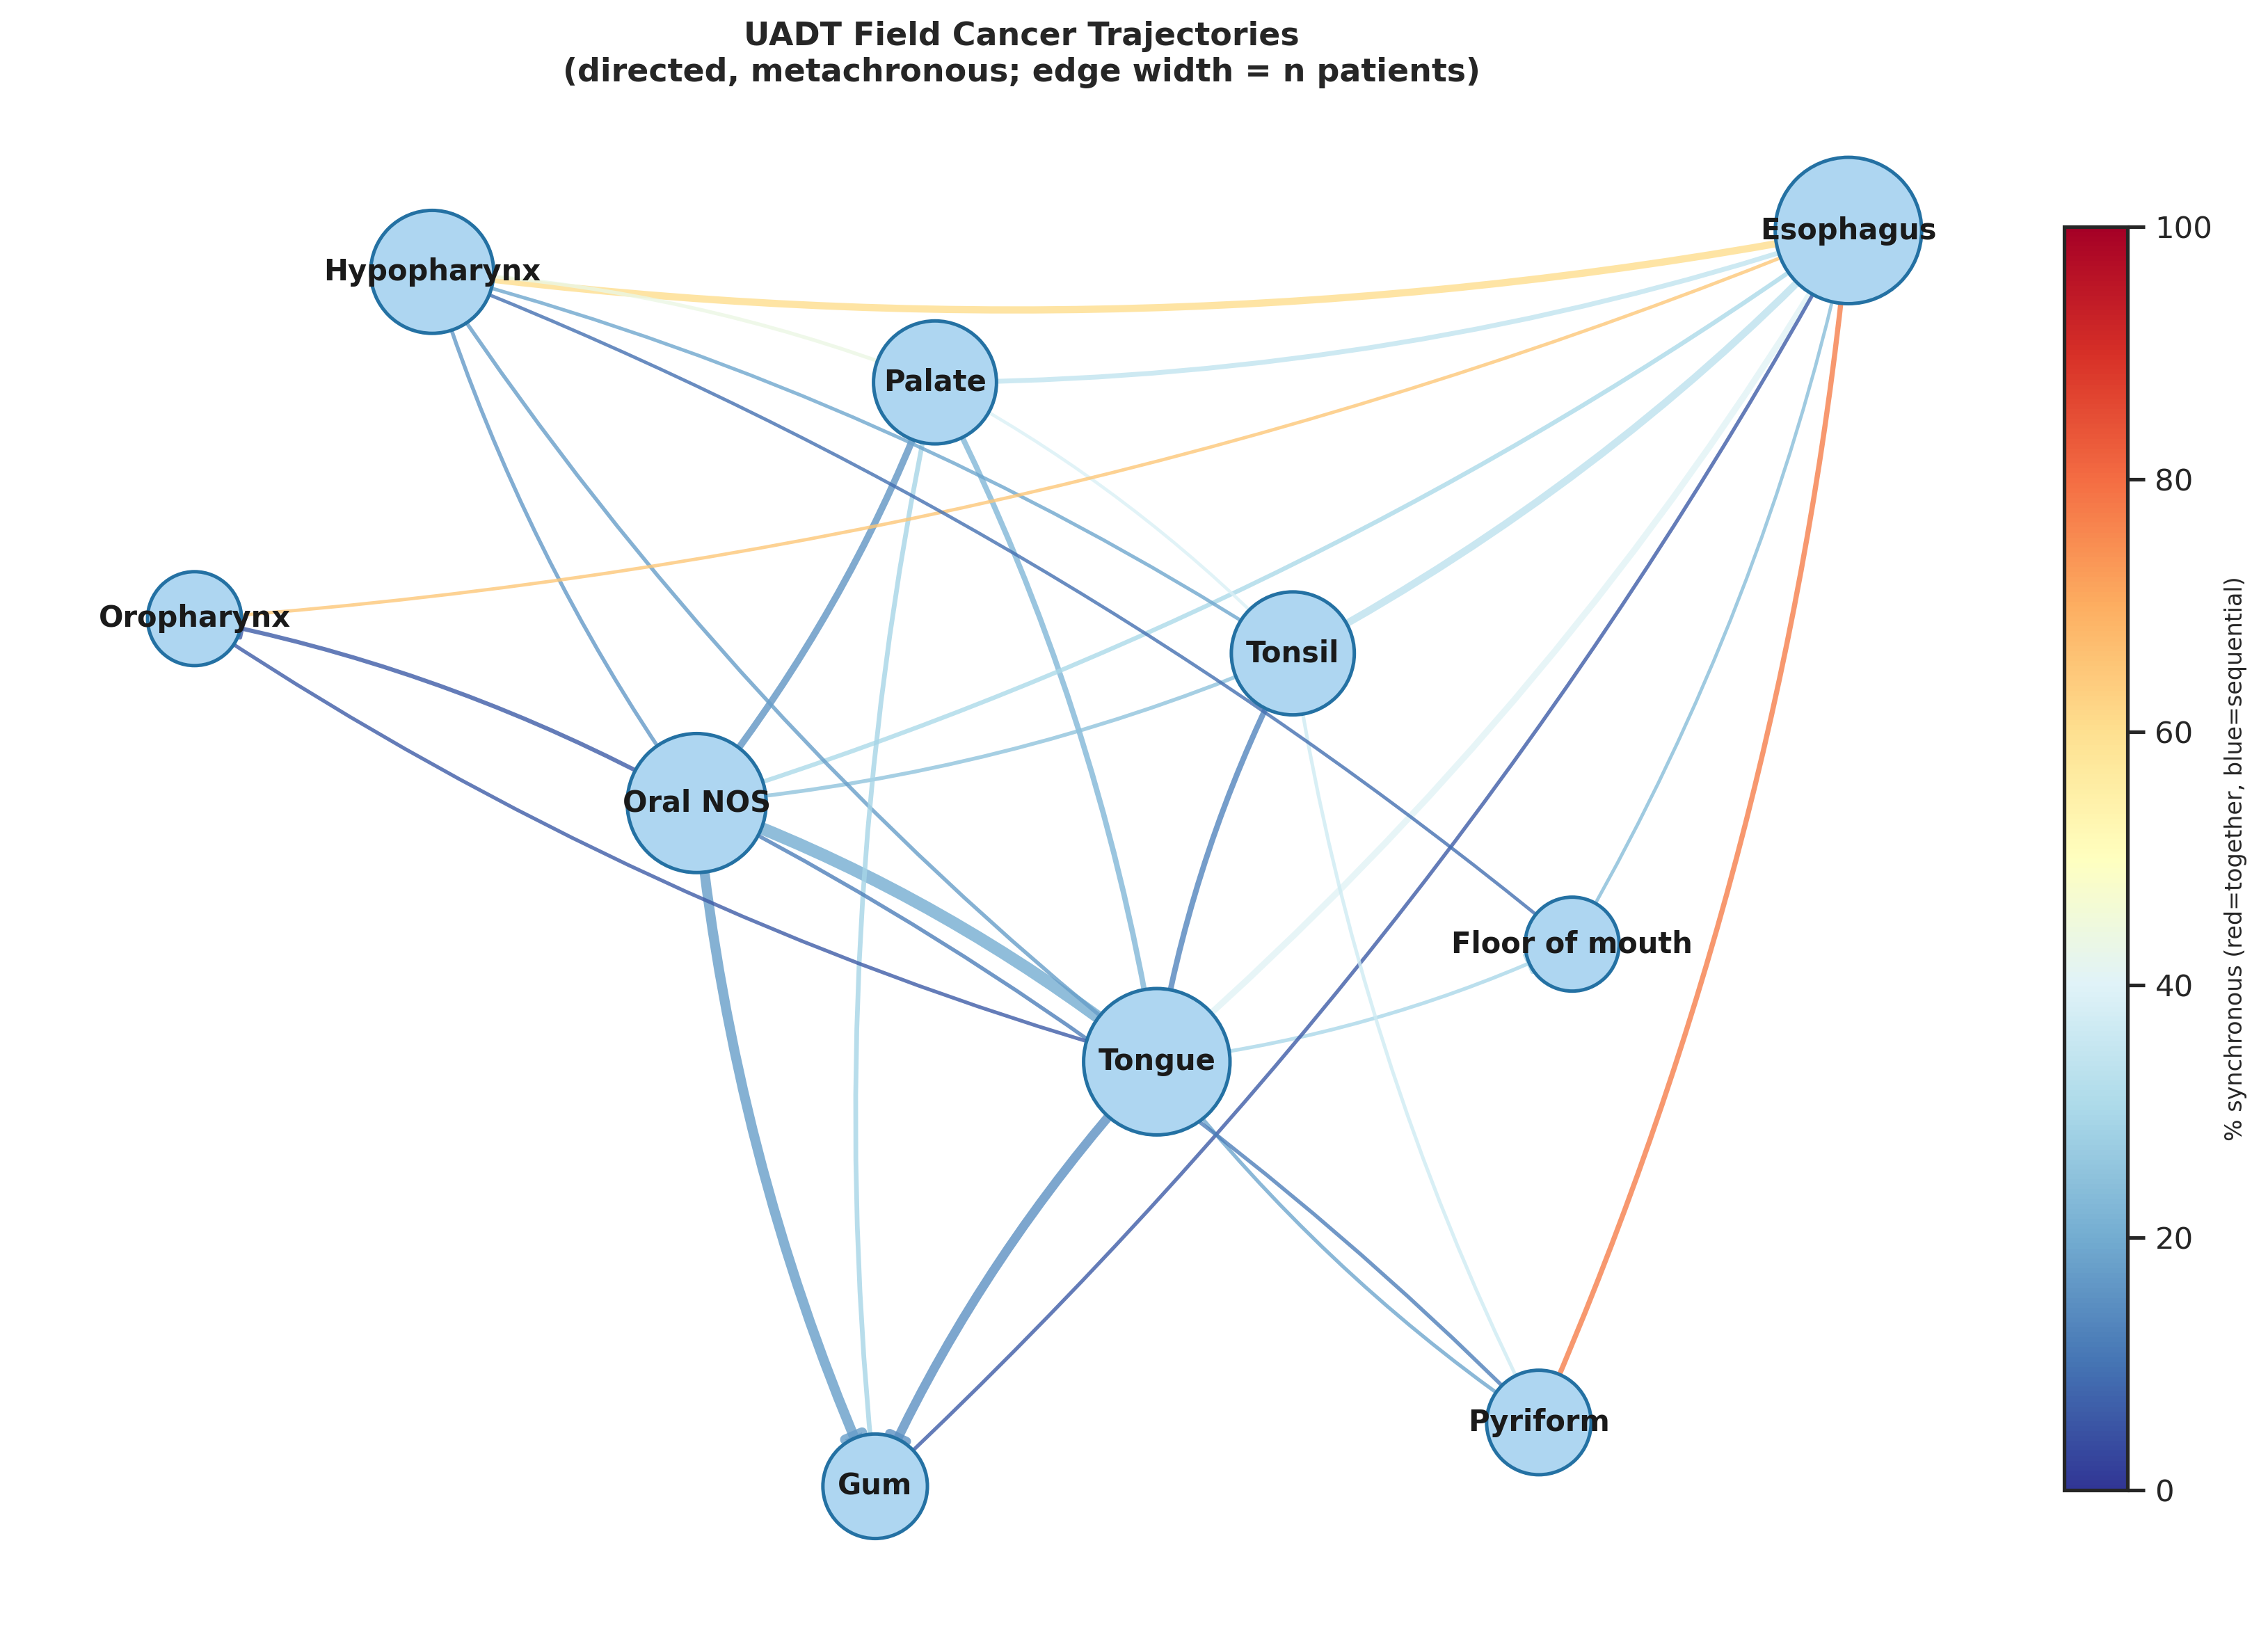
\includegraphics[width=0.9\textwidth]{fig4a_trajectory_graph.png}
  \caption{\textbf{Directed transition network.}
  Nodes represent UADT field sites; directed edges represent observed first-to-second
  cancer transitions. Edge width is proportional to the number of transitions.
  Edge colour encodes the \textit{synchronous fraction}: the proportion of
  transitions for that directed pair in which the second diagnosis occurred within
  6 months of the first (scale: light blue\,=\,0\% to dark navy\,=\,100\%;
  colorblind-safe sequential palette).
  The bidirectionality of the pyriform--esophagus and
  hypopharynx--esophagus arcs (symmetry score\,=\,0.879,
  defined as $\min(n_{\mathrm{fwd}},n_{\mathrm{rev}})/\max(n_{\mathrm{fwd}},n_{\mathrm{rev}})$)
  supports a field mechanism rather than directional spread.}
  \label{fig:trajectories}
\end{figure}

\begin{figure}[ht]
  \centering
  \begin{minipage}{0.48\textwidth}
    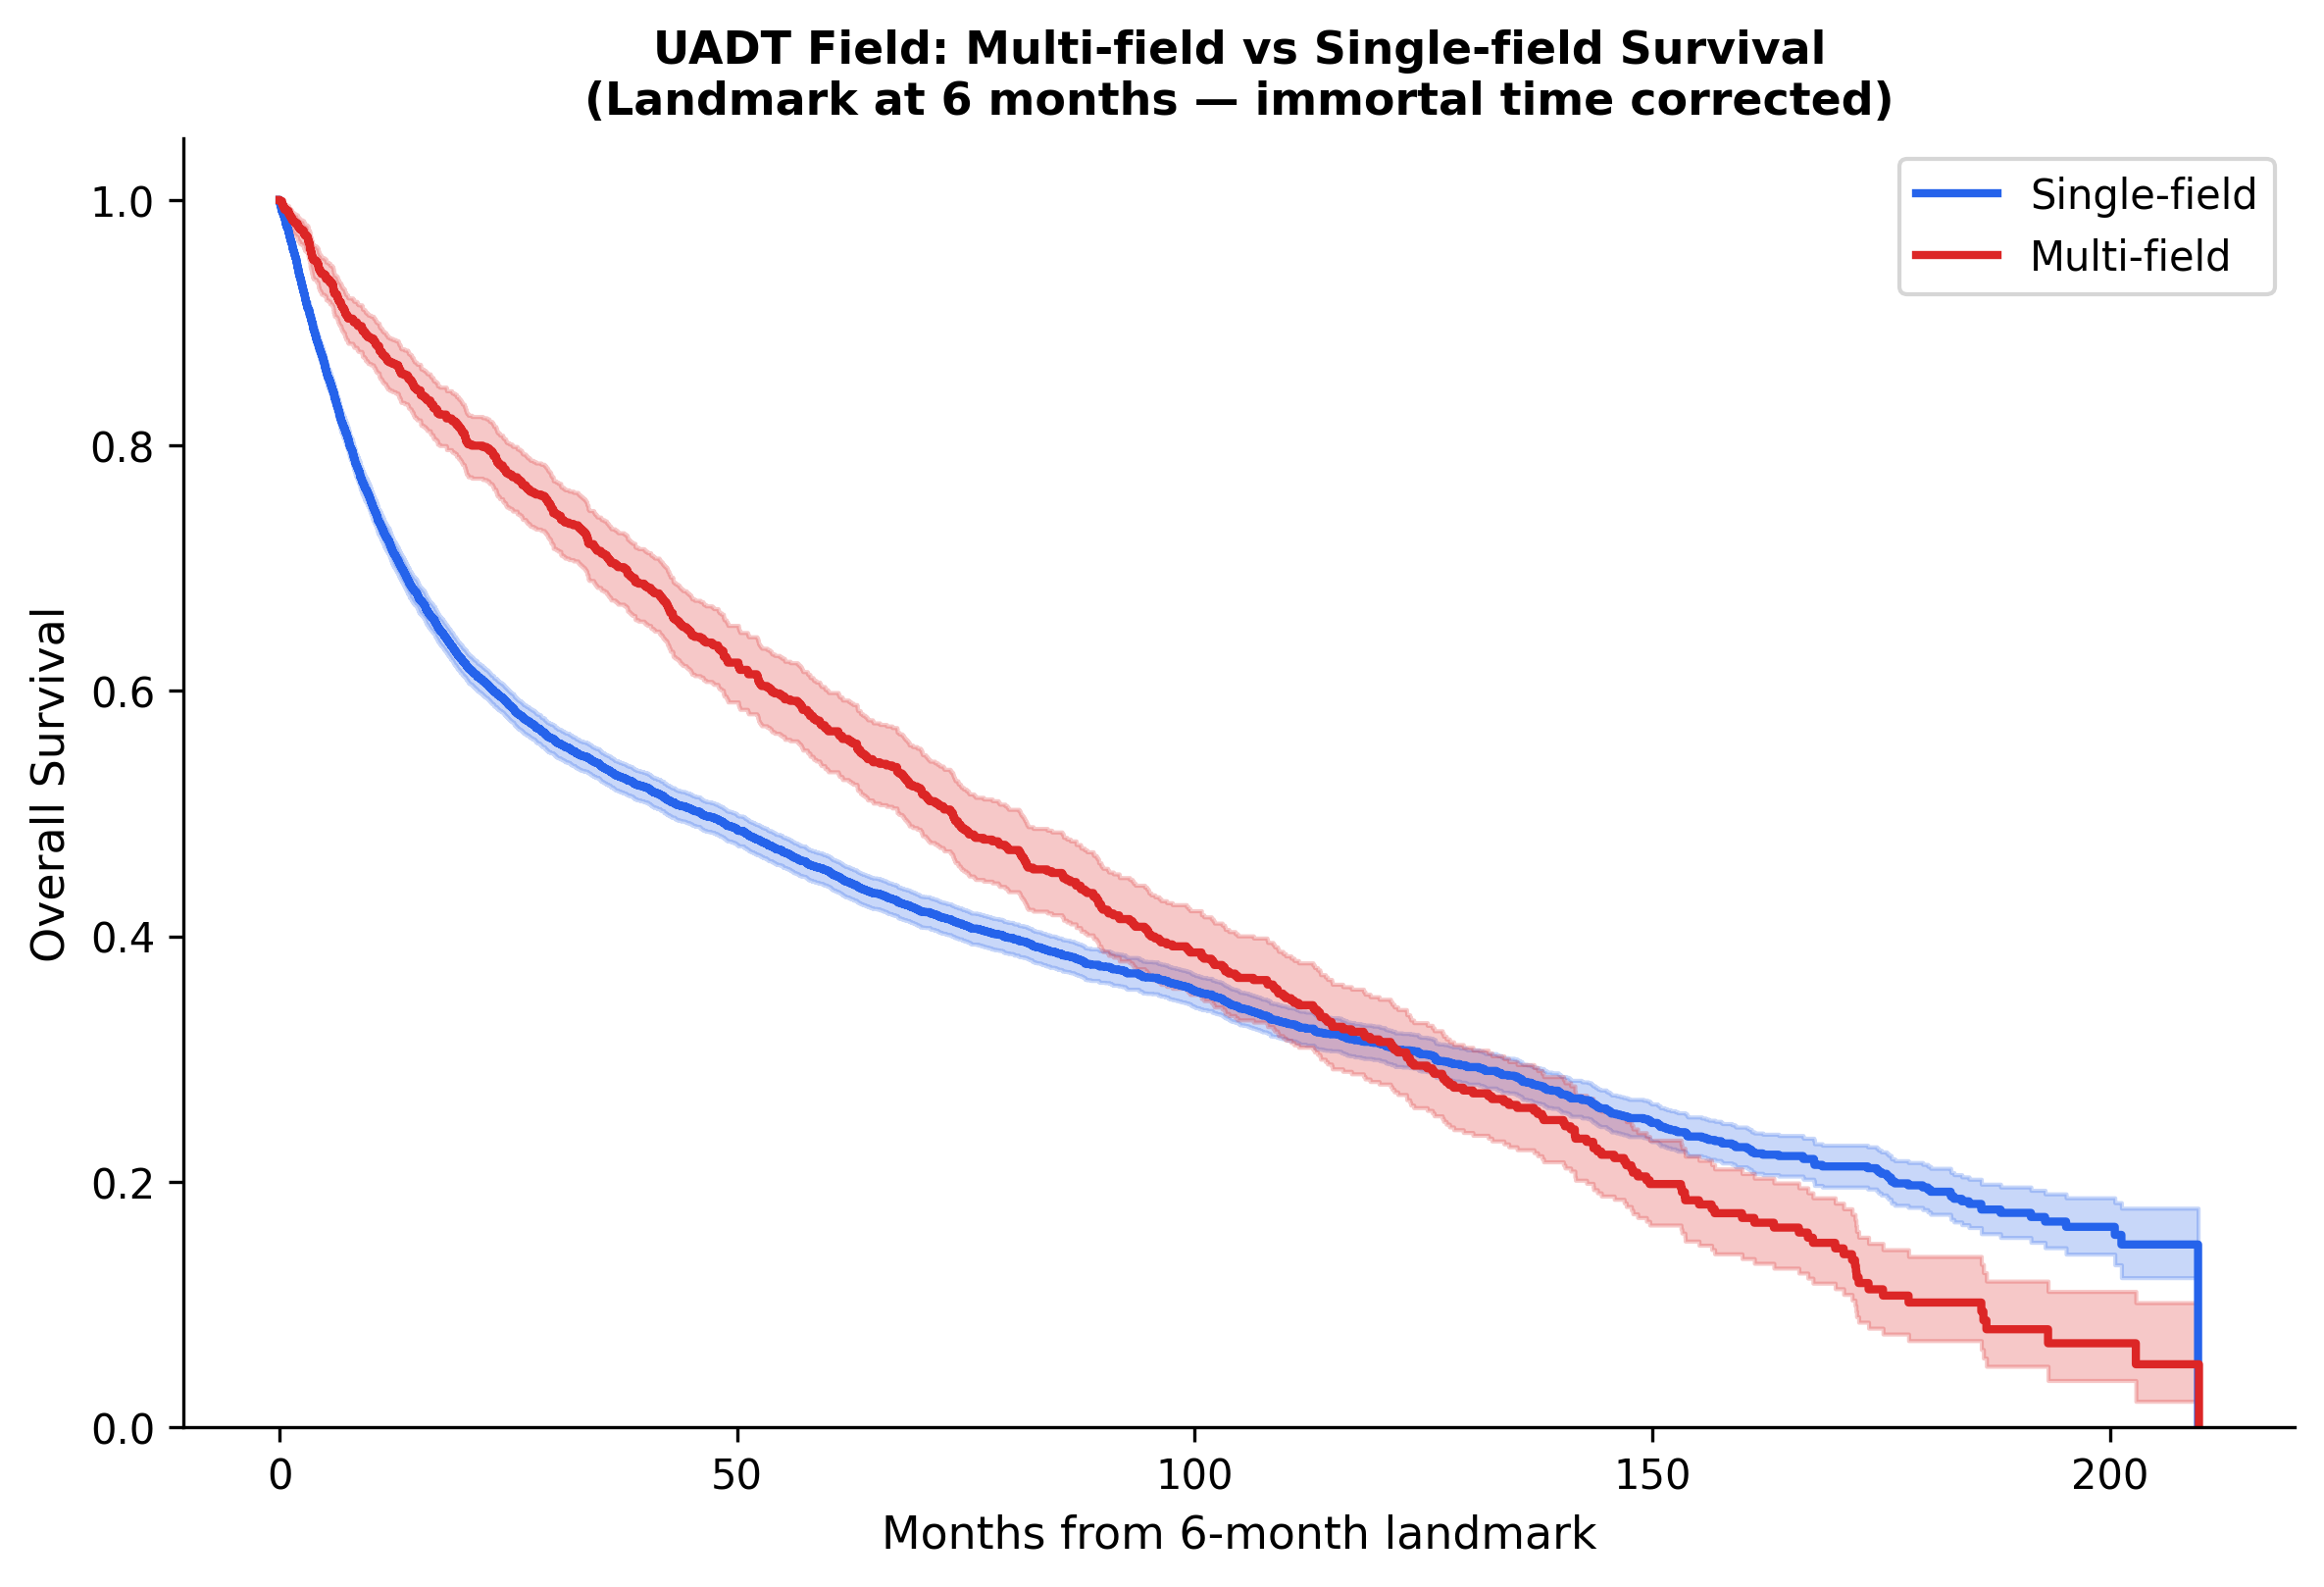
\includegraphics[width=\textwidth]{fig5a_km_landmark.png}
  \end{minipage}\hfill
  \begin{minipage}{0.48\textwidth}
    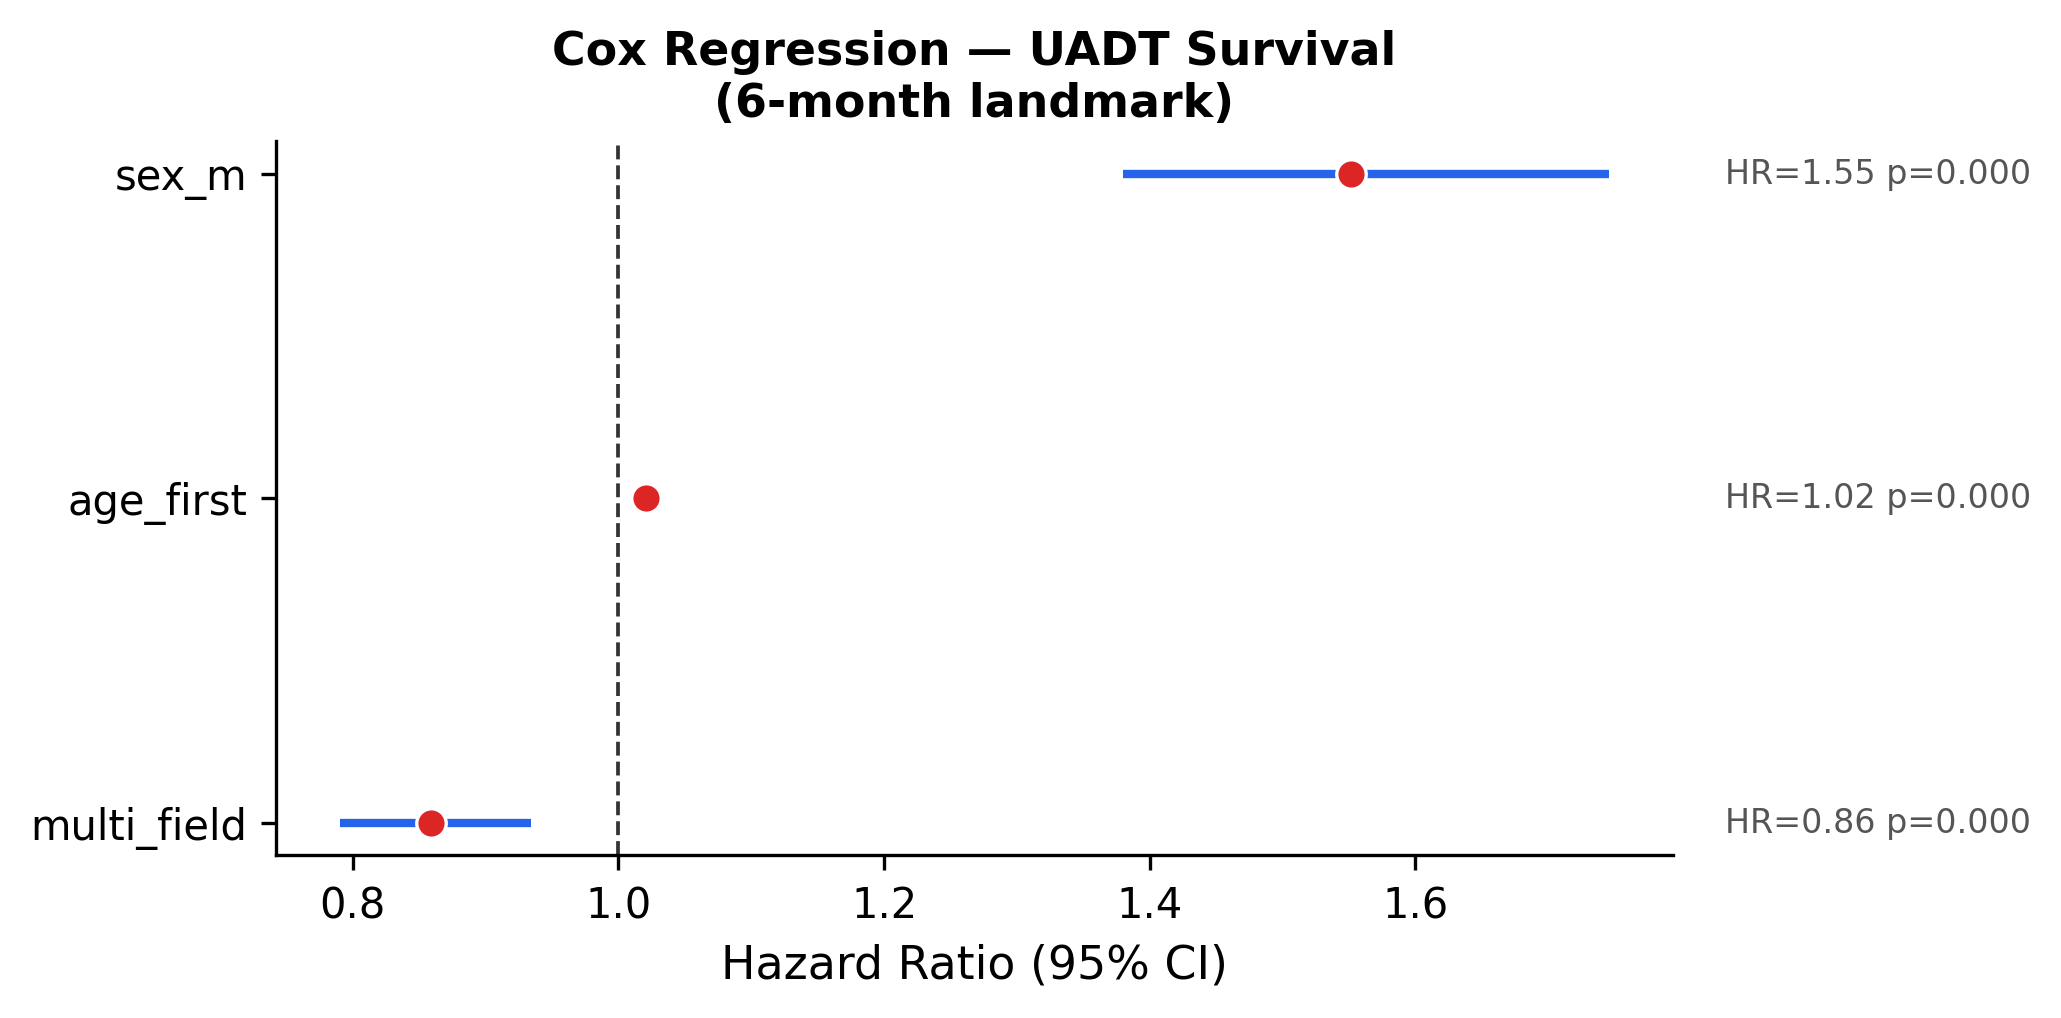
\includegraphics[width=\textwidth]{fig5b_cox_forest.png}
  \end{minipage}
  \caption{\textbf{Survival impact of multi-site UADT disease.}
  \textit{Left:} Kaplan--Meier curves for single-site (grey) versus multi-site
  (red) UADT patients after 6-month landmark; the apparent protective effect
  is an immortal-time artifact.
  \textit{Right:} Forest plot from time-varying Cox regression (HR\,=\,2.14,
  95\%\,CI\,1.97--2.33); multi-site exposure is coded as a time-varying indicator
  turning on at the date of second UADT diagnosis.}
  \label{fig:survival}
\end{figure}

\begin{figure}[ht]
  \centering
  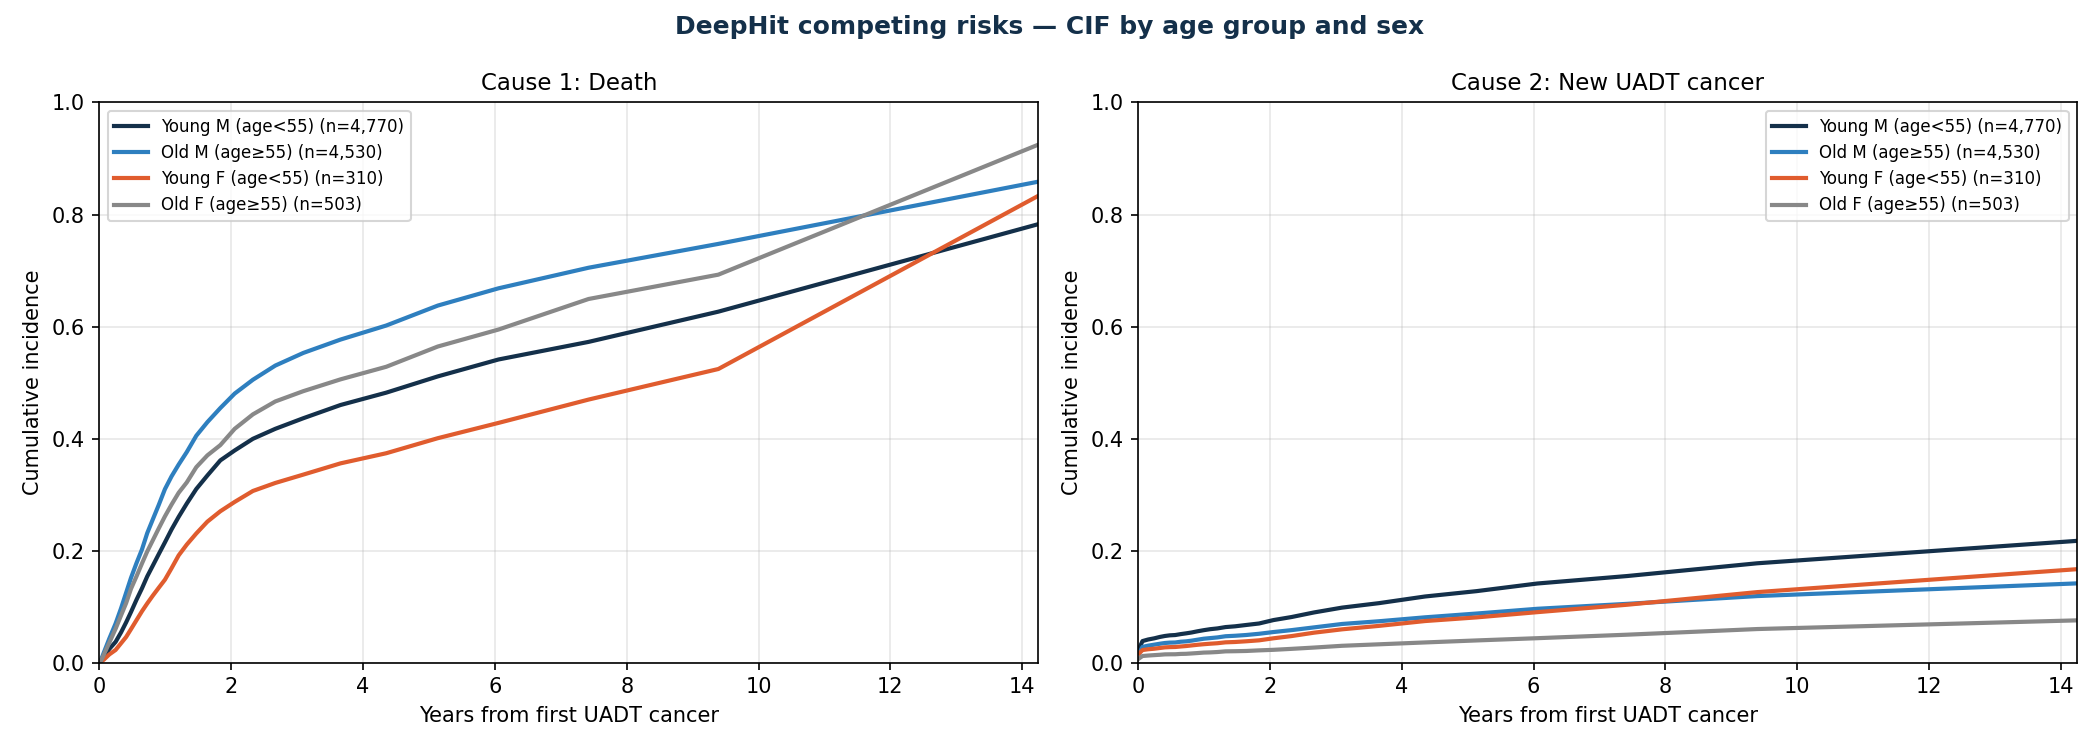
\includegraphics[width=0.95\textwidth]{fig_cif_curves.png}
  \caption{\textbf{Competing-risks cumulative incidence functions (CIF).}
  Mean CIF for cause~1 (death, left panel) and cause~2 (new UADT cancer, right panel)
  estimated by DeepHit, stratified by age group and sex.
  At 5 years: overall death CIF 56.7\%; second UADT cancer CIF 10.4\%.
  Death dominates at all time horizons, supporting immediate initiation of
  surveillance rather than deferred screening.}
  \label{fig:deephit}
\end{figure}

% ── Supplementary note ────────────────────────────────────────────────────────
\newpage
\section*{Supplementary Methods}

\subsection*{Pre-registration of hypotheses and field definition}

The following hypotheses and constants were declared in code before any
registry data were loaded:

\begin{enumerate}
  \item \textbf{PRIMARY:} The pyriform sinus -- esophagus and
    hypopharynx -- esophagus pairs have the highest co-occurrence rates
    within the UADT field cohort.
  \item \textbf{SECONDARY:} Hypopharynx -- esophagus transitions are
    bidirectional (symmetry score $\geq$ 0.80, binomial $p > 0.05$).
  \item \textbf{TERTIARY:} Multi-site UADT disease is associated with
    increased mortality (HR $>$ 1.0) after immortal-time correction.
\end{enumerate}

Field sites were locked as \texttt{FIELD\_SITES = [C02, C03, C04, C05, C06,
C09, C10, C12, C13, C15]} and the synchronous threshold as
\texttt{SYNC\_MO = 6} before any data loading occurred.

\subsection*{Immortal-time bias — landmark vs.\ time-varying comparison}

In the 6-month landmark analysis, all patients surviving beyond 6 months
were included, and \texttt{multi\_field} was coded as a fixed baseline
covariate (0 if second cancer occurred after landmark, 1 otherwise).
This approach does not fully eliminate immortal-time bias because patients
coded as \texttt{multi\_field\,=\,1} at baseline must have survived from their
first diagnosis to the second — a guaranteed survival interval not shared by
single-site patients.

The time-varying analysis eliminates this by splitting each patient's
follow-up record at the date of the second UADT diagnosis:
the interval before the second diagnosis contributes as
\texttt{multi\_field\,=\,0}; the interval after contributes as
\texttt{multi\_field\,=\,1}.
This counting-process formulation is the gold standard for time-dependent
exposures in survival analysis~\citep{suissa2008,therneau2013}.

% ── References ────────────────────────────────────────────────────────────────
\newpage
\bibliographystyle{unsrt}
\bibliography{references}

\end{document}
